\section{Implementation}
%------------------------
In this sprint we have created a very naive implementation of the utility. It supports the most basic types of C-structs. In addition the utility supports some basic configuration.

We have decided to use YAML as our configuration format. In this sprint we have added support for range specification.
A user can specify the ranges of the members of a struct, from a minimum to a maximum.
In the screenshot below you can see how Wireshark displays a member that has an invalid range. \newline
\begin{figure}[here]
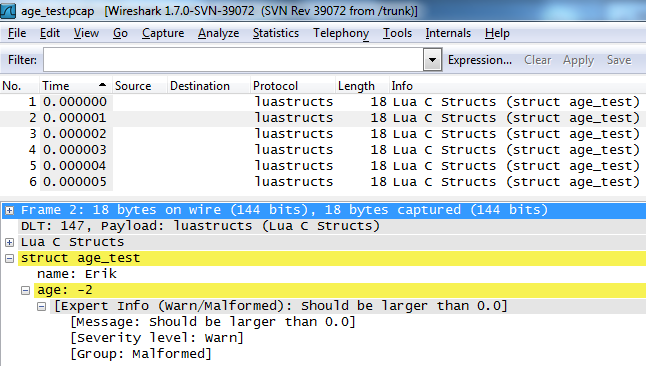
\includegraphics[width=1.2\textwidth]{pics/wireshark_outofrange}
\caption{Wireshark dissector}
\label{fig:dissector_screenshot}
\end{figure}	

The tool uses a command line interface. The user inputs a header-file and optionally a configuration file to the command line, and the program outputs a Lua-script.  Below you can see a figure that illustrates how the program is run.
\begin{figure}[here]
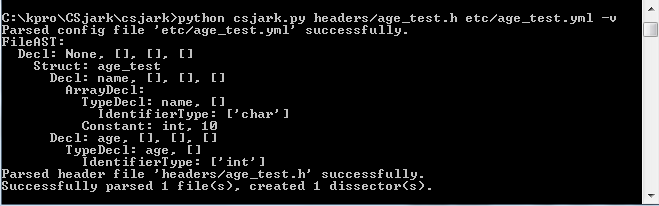
\includegraphics[width=1.2\textwidth]{pics/cmd_agetest_run}
\caption{Command line}
\label{fig:cmd_screenshot}
\end{figure}

